\chapter{Methods}

\section{Markov Models}

\subsection{Expected Number of Substitutions}

\section{Data Sets}

To establish the properties of my methods on alignments that range in their evolutionary divergence, I sampled a widely used molecular marker of genetic diversity. Herein the Microbial data, this is a subset of GreneGenes, a database of consistent alignments of the 16S rRNA gene in microbes. The Microbial data consists of 9702 alignments with a uniform distribution of Jensen-Shannon Divergence (JSD), details of the sampling process are described in Kaehler \textit{et al.} \cite{Kaehler2015}. 

Data for the Primate data set was sampled from Ensembl release 104 \cite{Howe2021Ensembl2021}. 



Ensembl Compara \cite{Howe2021Ensembl2021} contains annotated genome-wide species comparison data. This resource provides valuable annotation of related sequences amongst species, primarily vertebrates. 


The annotation of orthologs in the data set is done through the following pipeline. 

\section{Simulation Study}

\subsection{Choosing Seed Alignments}
I require alignments simulated in accordance with a GNS process. One way to obtain data evolving under a GNS process is to exploit the fact that even a non-stationary process will converge to its stationary nucleotide distribution (herein $\pi_{\infty}$) as time goes to infinity. Essentially, I can obtain a GN model from real data, derive its corresponding $\pi_{\infty}$ and use those two things to define a stationary process. The process can be modified to model the background edges as discrete, and I can simulate alignments according to such a specification. This is my chosen simulation method as the resulting alignments are generated from parameters of real data. 

I must consider how the properties of the alignment used for simulation may affect the application of my methods. To address this requires deciding the features of an alignment that may be significant and finding measures that characterise them. I can then choose a selection of alignments that vary systematically by these measures. From each alignment, I can create a data set, resulting in a collection of data sets that differ in a way that reflects the natural variation of real sequence data. Using carefully diversified data allows for a thorough interrogation of my methods and determines how their properties may change when applied to different types of data.

An important measure I require is that of non-stationarity. A direct consequence of a non-stationary process is a change in base composition over time. As follows, an indication of the degree of non-stationarity can be obtained from the difference in compositions between sequences in the same alignment. It is worth noting that studies of compositional data often require representation using Aitchison geometry. This representation allows for a consideration of the vulnerability of a composition to the sample it comes from. However, the composition of bases can also be considered as a probability distribution (i.e., $\pi = [\pi_T,\, \pi_G, \, \pi_C, \, \pi_A]$, such that $\pi_i$ where $i= \mathrm{T}, \mathrm{G}, \mathrm{C}, \mathrm{A}$ is the probability of observing the state $i$). In the case of comparing probability distributions, several measures can be used. My selected measure is an information theoretic measure known as Jensen-Shannon Divergence (JSD). JSD measures the similarity between probability distributions. JSD was chosen as it can accommodate multiple distributions, allowing us to apply it to more than two sequences if needed. Additionally, it has an associated true metric, satisfying important mathematical properties (e.g., the triangle inequality). 

A probability distribution also has an associated information content, measured using entropy. Entropy is a fundamental quantity that indicates, in our case, the evenness of base composition. For example, $\pi =[1,\, 0,\, 0,\, 0]$  (a single nucleotide) has zero entropy whilst  $\pi =[0.25,\, 0.25,\, 0.25,\, 0.25]$ (equifrequent nucleotides) has the maximum possible entropy for 4 states. As a measure of compositional diversity, it captures an essential feature of the mode of evolution. For example, an edge that is highly \gls{strand-asymmetric} would have lower entropy than a \gls{strand-symmetric} edge. The base composition may affect the properties of my developed methods. One example being $T_{50}$ for which base composition is used in its computation. Accordingly, the impact of compositions with different entropy is an important feature to consider in the process of method development.

I will approximate the stability of the process using the condition number of the foreground rate matrix. It is important to derive data from numerically stable processes. If a process falls within the scope of being numerically unstable, (meaning computers are poorly equipped to evaluate it using standard settings), I need to be aware of this so I can select a more numerically stable method. An indication of numerical stability is the eigenvector matrix condition number. A matrix condition number is an approximation of the worst case relative change in derivations, for a relative change in the input. For a continuous-time process, the transition rate matrix $\mathrm{Q}$, specifies the instantaneous rates of exchanges between states. $\mathrm{Q}$ is foundational to a given substitution model. The eigendecomposition of $\mathrm{Q}$ is a representation of $\mathrm{Q}$ in terms of its eigenvalues and eigenvectors. Eigendecomposition is fundamental to many methods that I am using and developing (e.g., deriving $\pi_{\infty}$). As an indication of the suitability of a matrix to decomposition, I will use the eigenvector matrix condition number to approximate the numerical stability of a process.

I chose four microbial alignments to generate synthetic data sets and refer to these as seed alignments. As previously stated, I expect that JSD, entropy, and condition number may affect the numerical and or statistical properties of the developed methods. To derive data from numerically stable processes, the seed alignments are chosen from a subset of alignments where the eigenvector condition number is low ($<1.5$). To capture the extent of naturally occurring diversity (measured by JSD) and compositional diversity (measured by entropy), the seed alignments chosen represent the permutations of those extremes. These are: high JSD, low entropy; high JSD, high entropy; low JSD, low entropy; low JSD, high entropy. 

\subsection{Generating Synthetic Alignments that are Stationary, but not Reversible}
I expect the properties of my test to be affected by the number of substitution events that distinguish the sequences in an alignment. The mathematical proof that LRT statistics are $\chi^{2}$ distributed assumes infinite data, that is the alignment is infinitely long. Although it has been shown that a few hundred base pairs can be sufficient for the $\chi^{2}$ to be accurate, this length is ultimately dependent on the number of substitution events \cite{Ota2000AppropriateParameters}. I can increase the number of events in a simulated alignment in two ways, (1) increase the length of the alignment, (2) increase the \gls{branch length} of the tree (increased divergence time). 

It is necessary to determine how my methods are affected by the length of the alignment. I have done this by simulating multiple data sets differing in alignment length for all four seeds. The lengths were chosen to be representative of alignment lengths of my biological application. The shortest sequences I will be using are protein coding genes, for which the average length (using just the 3rd codon position) is about 300bp. For each of the four seeds, I generated data sets of alignment length 300, 3,000, and 30,000.   

It is also necessary to determine the influence of increased branch length. When simulating alignments, I can alter the branch lengths of the generating function. This is a capability that allows me to create synthetic alignments specified by the same process (same $\mathrm{Q}$), but with an increased term of divergence. To address how branch length affects the test, I simulated data sets with an increased branch length for all four seeds. The genetic distance ($d$) (or branch length) is a measure of the expected number of nucleotide substitutions per site. The maximum branch length in my application data sets will be about $d=0.6$. For the long branch simulations, I scaled the tree by a factor of 3. However, branch lengths were capped at $d=0.6$ and the remaining branch lengths were reduced proportionally. 

Each simulation set consisted of 1,000 synthetic alignments. The synthetic alignments are generated from the same function, derived from the parameter estimates from one seed alignment. The simulation process that was performed is described in Figure \ref{fig:simulating_alns}.

\begin{figure}[!ht]
\centering
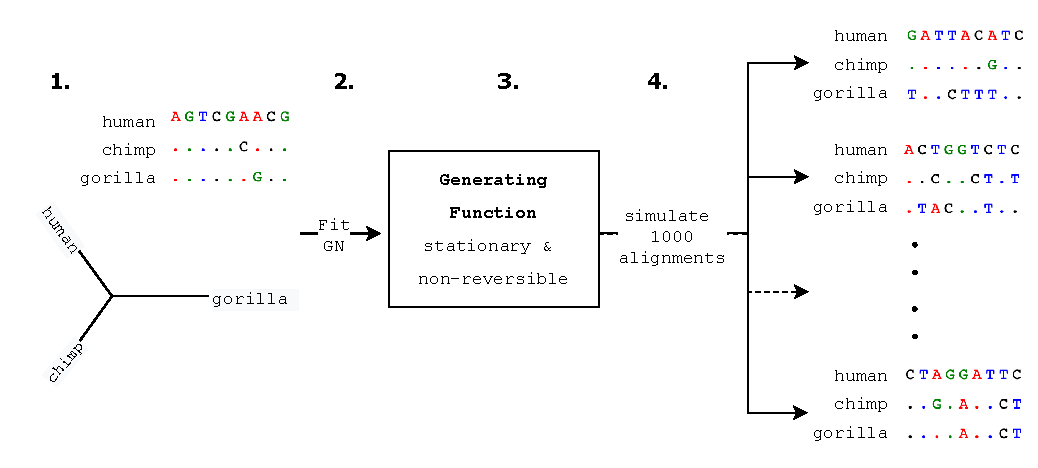
\includegraphics[width=\textwidth]{figures/diagrams/simulating_alns.pdf}
\caption{Creating synthetic data sets whose evolution was stationary but not reversible. \textbf{1,} select seed alignment, \textbf{2}, fit GN mixed model and extract model parameter estimates, \textbf{3}, define generating function using parameter estimates altered to be stationary, \textbf{4}, generate 1000 alignments of length $n$ and branch length scaled by $b$. For all 4 seeds this was performed for n = 300, 3000, 30000, and for each n, b = 1 and 3.}
\label{fig:simulating_alns}
\end{figure}

\section{Test for Disequilibrium}

To achieve this aim I have designed a Likelihood Ratio Test (LRT). The predominant method for examining aspects of sequences' evolution is through the use of \glspl{Substitution model}. \Gls{Maximum Likelihood} methods allow for measuring the support for a hypothesis, (in this case, a \gls{model}), given some data. Whether one hypothesis is better supported than another can be evaluated by using an LRT. Two models fundamental for my LRT are General Nucleotide (GN) and General Nucleotide Stationary (GNS). Their point of difference is that the parameters of a GNS rate matrix must satisfy $\pi\mathbf{Q}=0$, i.e., the process is constrained to be stationary (and thus in equilibrium). Consider an LRT in which GNS is the null and GN is the alternate. If we reject the null, we may conclude that the sequences are more likely to have been generated by a process which is not yet stationary, as this is the only component unique to the alternate.

An LRT as described above is too naive for my objective to test for equilibrium in a single lineage. For a model to be \gls{identifiable} requires an alignment of at least three sequences \cite{Chang1996FullConsistency}. Consequently, a significant result for such an LRT will not reveal which of the taxa is causing the rejection of the null. To test for disequilibrium in a single \gls{edge} requires  modelling a continuous-time process on the edge of interest (herein the foreground edge) and assuming discrete-time processes for the other edges (herein the background edges) \cite{Verbyla2013TheSubstitution}. A discrete-time process is more general (fewer assumptions) than even the GN, making it the ideal background. 

Using mixed discrete- and continuous-time Markov processes, I can test for disequilibrium on a single edge. For such an LRT, the foreground edge assumes GNS for the null, and GN for the alternate. Both hypotheses assume a Barry and Hartigan (BH) model, the most commonly implemented discrete-time process, for the background edges. The modelling of the foreground edge, set apart by the assumption of stationarity, is the only point of difference between hypotheses. For this LRT, a rejection of the null means that the foreground edge was described significantly better with a non-stationary process. Such a result suggests disequilibrium precisely in the foreground edge. Put explicitly, the test will be between the following hypotheses:\\ $\mathbf{H_0}$: the foreground evolved according to the \textbf{GNS}, the background according to BH. \\ $\mathbf{H_1}$: the foreground evolved according to the \textbf{GN}, the background according to BH.\\
\noindent Herein all model fits assume mixed discrete- and continuous-time Markov processes, and a BH process is always assumed for the background edges. For brevity, I will refer to a model by the process assumed on the foreground edge.

\begin{figure}[htbp]
\centering
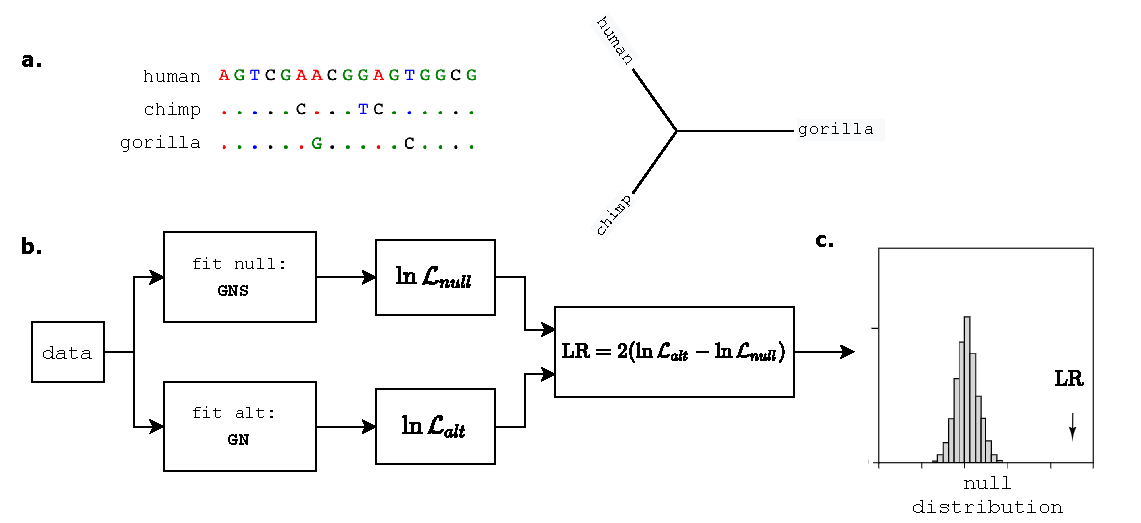
\includegraphics[width=\textwidth]{figures/diagrams/LRT.pdf}
\caption{\textbf{Likelihood Ratio Test.} \textbf{a}, The data: an alignment of orthologous sequences for human, chimp and gorilla, and a phylogenetic tree indicating the relationship between taxa. \textbf{b}, A LRT comparing substitution models, GNS is the null and GN is the alternate. The log-likelihood ($\ln\mathcal{L}$) for each model is obtained via fitting. The likelihood ratio (LR), is the ratio of the $\ln\mathcal{L}$ of the two models. \textbf{c}, the LR statistic is compared to the null distribution. In this case the statistic exceeds the distribution of values we would expect if the null was true, we would thus conclude that process is described significantly better with the alternate (GN) process.}
\label{fig:lrt}
\end{figure}

It is important that the best possible methods of model fitting are chosen. Recall that a necessary precursor to any application of my test is to establish maximal fits of the models. Additionally, the process of fitting a model to an alignment is the most time-consuming method routinely used in my project. I have sought to identify the quickest possible method that yields a maximised likelihood. 

For this, I conducted an initialisation experiment that makes use of a property of \gls{nested} models. For nested models, it is guaranteed that the likelihood for the alternate will be greater or equal to that for the null. General Time-Reversible (GTR) is the most general time-reversible process, and is required for my initialisation experiment. GTR is nested in GNS, which in turn is nested in GN. When a model is not maximally fit, the optimisation methods have failed to find the global maximum. Such is referred to as a local maximum, where they are higher points elsewhere but not nearby. In such cases, getting parameter estimates from a nested model fit to use as initial estimates may aid the optimisation in escaping a local maximum. I also wish to establish whether there is a speed gain in initialised model fits compared to uninitialised fits. Theoretically, if given starting values close to the optimal, this may reduce the time it takes to get there. 

For all synthetic data sets, I tested whether initialisation improved the model fitting process. The initialised method fit models in order of increasing generality (GTR, GNS, GN). Importantly, parameter estimates for each model were obtained from the previous model. The uninitialised method fit GNS and GN separately. The maximum likelihood estimates between uninitialised and initialised fits were compared for the models (e.g., uninitialised GN vs initialised GN). The time taken for each fitting process was recorded.  

The initialisation experiment revealed that there are no intrinsic problems with the fitting process for GN or GNS. A fit was considered non-maximal if the log-likelihood from the initialised method was higher than that of the uninitialised method. There were no occurrences of non-maximal fits for any of the synthetic alignments. Initialised fits which were faster than the corresponding uninitialised fits were rare, occurring at a rate of about ~1\%. These results suggest that the best method of fitting for both models is without initialisation. 



\section{Bootstrapping Data}




\section{Algorithmic Implementation}

